\subsection{Leapfrog}

\subsection{Potential and kinetic energies}
    \begin{lstlisting}
        void calc_energies(particle *p, int ntot, double *ekin, double *epot) {
          double sum_pot = 0, sum_kin = 0;
        
          for (int i = 0; i < ntot; i++) {
            sum_pot += p[i].pot;
            for(int k = 0; k < 3; k++) {
              sum_kin += p[i].vel[k] * p[i].vel[k];
            }
          }
        
          *ekin = 0.5 * sum_kin / ntot;
          *epot = 0.5 * sum_pot / ntot;
        }\end{lstlisting}

    \begin{equation}
    	T=\frac{1}{k_B}\langle E\rangle \qquad
        \Rightarrow T'=\langle E'\rangle
    \end{equation}

    \begin{figure}[h!]
        \centering
        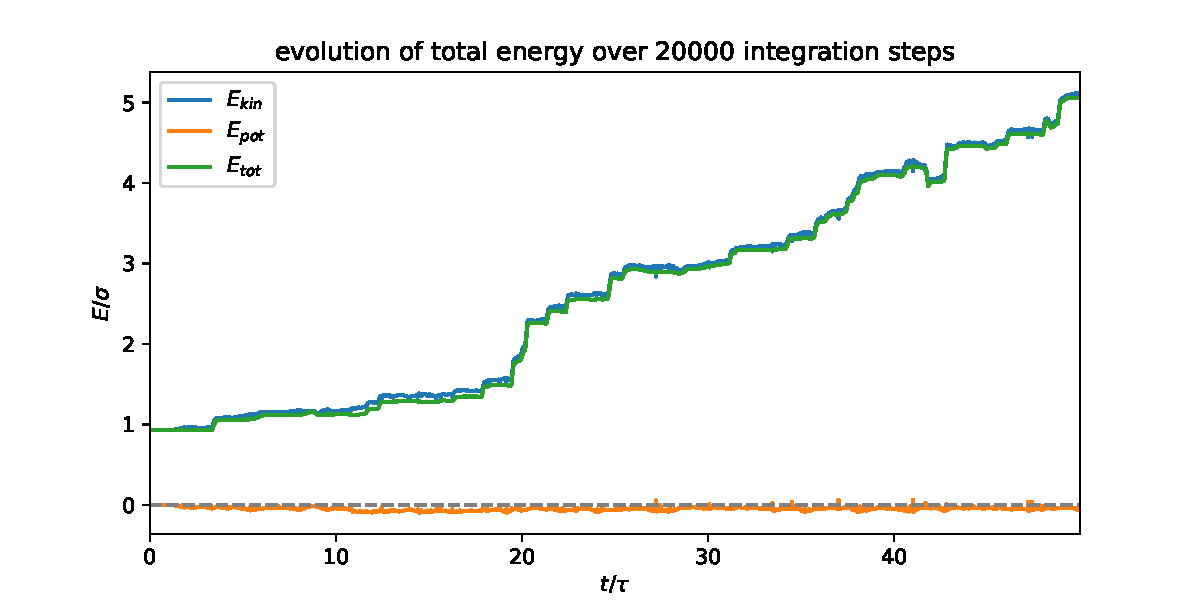
\includegraphics[width=\textwidth]{../figures/energy.pdf}
    \end{figure} \ \\ 
    \begin{itemize}
        \item jumps in energy
        \item maybe related to close-encounter events? \\
            $\Rightarrow$ ignore interactions between very close particles
        \item with $d_{min}=0.1$: smaller jumps than with $d_{min}=0.01$,
            which again are smaller than without setting $d_{min}$ at all 
            (i.e. taking all interactions into account).
    \end{itemize}

